\problemname{Magic Marbles}

\illustration{0.32}{marble}{A frozen marble on ice. Image by rihaij, \href{https://pixabay.com/photos/ice-bubble-bubble-soap-frost-bubble-6020105/}{Pixabay}\vspace{-0.5cm}}
You may know \emph{Wizard's Chess}, which is a magical version of chess, but there are more magical games in the wizarding world.
Another one you may recognize is \emph{Magic Marbles}, which is similar to the muggle game \emph{Marble Temple}.
In this game, you are given a chain of differently coloured marbles~$m$, which you need to destroy.
To do this, you can add additional marbles to the chain.
This may sound counterproductive, but if there ever is a \emph{run} of at least~$k$ consecutive marbles that are of the same colour, then all of these marbles magically disappear instantly.
The resulting gap is closed by moving the remaining marbles closer together, which can lead to new runs that then again disappear.

\begin{figure}[!h]
	\centering
	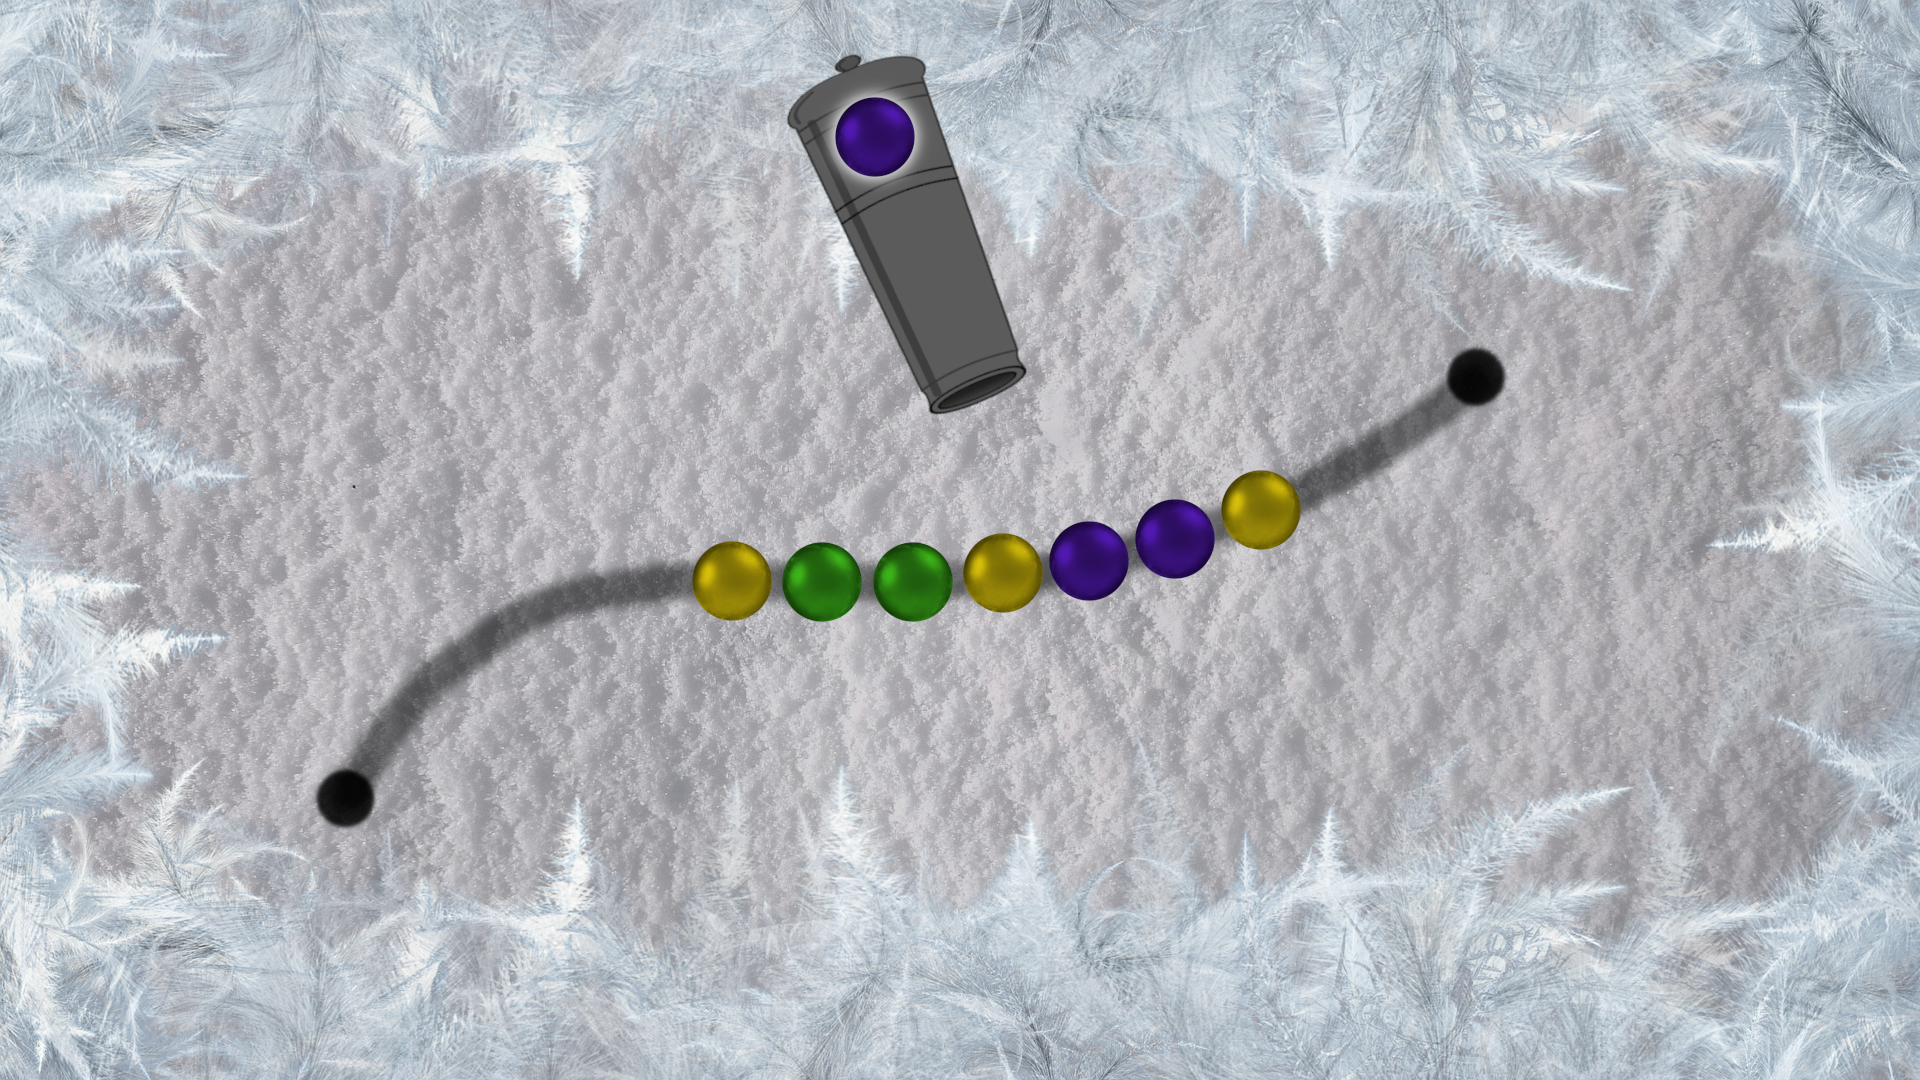
\includegraphics[width=0.5\textwidth]{sample}
	\caption{The initial state of the first sample.
	The first marble will be added between the second yellow marble and the first blue marble.
	Since this results in a run of three blue marbles, all of them instantly disappear.}
\end{figure}

This year there is a great Magic Marbles tournament in Hogwarts.
However, you fear that some magicians are not as sincere as you and may try to cheat in this magic tournament.
Therefore, you decided to simulate the game without magic.

\begin{Input}
The input consists of:
\begin{itemize}
	\item One line with three integers $n$, $k$, $q$ $(1\leq n,q\leq2\cdot10^5, 2\leq k\leq4\cdot10^5)$, the initial length of the marble chain $m$, the minimal run length where marbles disappear, and the number of marbles that will be added during the game.
	\item One line with $n$ space-separated integers $m_i$ $(1\leq m_i\leq10^6)$, where $m_i$ is the colour of the $i$-th marble of the initial chain $m$.
	It is guaranteed that each run of marbles of the same colour has length less than $k$.
	\item $q$ lines, each containing two integers $p_x$ and $m_x$ $(0\leq p_x \leq |m|, 1\leq m_x\leq10^6)$, the position where the next marble will be inserted and the colour of the marble that is inserted.
	$|m|$ denotes the current length of the marble chain.
	If the position $p_x$ is $0$, the marble will be added in front of the currently first marble. Otherwise, the marble will be added after the $p_x$-th marble.
\end{itemize}
\end{Input}
\begin{Output}
For each of the $q$ insertions of a new marble, output a single integer $|m|$, the length of the marble chain after that insertion and any deletions that were caused by it.
\end{Output}
